\section{Methodology}
\label{sec:method}

% Restructured 12 Oct 2026 to the thesis plan of 11 Oct (section 4, "3 System and method"): 3.1 rig, twin and
% roles (system_overview.tex, with the twin from simulation.tex); 3.2 model and planner (model.tex, the planner
% part of controller.tex); 3.3 tracker, thrust map, measured pull, model integral, takeoff and landing
% (controller.tex, takeoff_landing.tex); 3.4 reconfiguration (reconfiguration.tex); 3.5 authority and safety
% (authority.tex, new; the safety paragraph and the owners figure); 3.6 method and metrics (simulation.tex as the
% protocol, trajectories.tex, metrics.tex). Earlier history: 9 Oct structure audit (hardware.tex split into
% system_overview, controller, Section 4.1, Appendix B and C, simulation.tex).

This section describes the rig, its twin and who flies what (Section~\ref{sec:overview}); the model and the
planner (Section~\ref{sec:model}); the tracker on each UAV, its thrust map, the measured rod pull, the model
integral, and the procedures that take a flight from the floor into the regime the model covers and back
(Section~\ref{sec:tracker}); the reconfiguration, in both directions (Section~\ref{sec:reconfig}); who owns each
UAV and what keeps the fleet safe when a step fails (Section~\ref{sec:safety}); and the experimental method with
the metrics every result is scored on (Section~\ref{sec:experiments}).

% system_overview.tex -- Methodology: system and platform (draft 4 Oct 2026).
% Restructured 9 Oct (structure audit): the platform paragraphs and fig:geometry moved here from
% hardware.tex, so the geometry is defined before the model; the duplicate reference and takeoff
% paragraphs cut (the interpolation sentence moved to the planner's output).

\subsection{System and platform}
\label{sec:overview}

\subsubsection{Nodes and safety}

All control runs centrally, on one ground computer under ROS~2 (Robot Operating System~2). Motion capture (OptiTrack) is the
only sensing. It gives the pose of each UAV and of the payload, and nothing on the payload is
instrumented. Each UAV's flight controller runs Betaflight in rate mode. It receives a collective
throttle and three body-rate stick commands over its own ExpressLRS (ELRS) radio link, and closes only its
inner rate loop. Figure~\ref{fig:nodes} shows the nodes and the information they exchange.

\begin{figure}[h]
\centering
\begin{tikzpicture}[>=Stealth,
    blk/.style={draw, thick, rounded corners=2pt, align=center, minimum height=0.95cm, font=\small},
    lab/.style={font=\scriptsize, align=center}]
  \node[blk, minimum width=2.4cm] (mocap) at (0,0) {Motion capture\\ \scriptsize poses};
  \node[blk, minimum width=2.7cm] (plan) at (4.9,0) {Load--cable planner\\ \scriptsize 10\,Hz};
  \node[blk, minimum width=2.4cm] (fm) at (9.5,0) {Fleet manager\\ \scriptsize phases, safety};
  \node[blk, minimum width=1.9cm] (op) at (13.4,0) {Operator};
  \node[blk, minimum width=2.7cm] (trk) at (4.9,-2.2) {Tracker $i$\\ \scriptsize 50\,Hz, one per UAV};
  \node[blk, minimum width=2.7cm] (uav) at (4.9,-4.4) {UAV $i$\\ \scriptsize ELRS link, Betaflight rate loop};
  \draw[->, thick] (mocap) -- node[lab, above] {payload\\ pose} (plan);
  \draw[->, thick] (mocap.south) |- node[lab, pos=0.75, above] {UAV pose} (trk.west);
  \draw[->, thick] (plan) -- node[lab, right] {horizon for UAV $i$} (trk);
  \draw[->, thick] (trk) -- node[lab, right] {throttle, rate sticks, magnet} (uav);
  \draw[->, thick] (fm) -- node[lab, above] {phase} (plan);
  \draw[->, thick] (op) -- node[lab, above] {commands} (fm);
  \draw[->, thick] ([xshift=-0.35cm]fm.south) |- node[lab, pos=0.75, above] {arm, disarm} ([yshift=0.18cm]trk.east);
  \draw[->, thick, dashed] ([yshift=-0.18cm]trk.east) -| node[lab, pos=0.25, below] {fault} ([xshift=0.35cm]fm.south);
\end{tikzpicture}
\caption[Nodes and links]{Nodes and links. Solid: commands, references and poses; dashed: a tracker
reporting a fault, which disarms the whole fleet. The operator's commands are ARM, TAKEOFF, LAND,
DETACH and ATTACH.}
\label{fig:nodes}
\end{figure}

The system has three layers.
\begin{description}
    \item[Planner.] The centralised load--cable MPC of Section~\ref{sec:controller}. At 10\,Hz it
    plans the motion of the payload and of every rod, and publishes to each UAV its reference over
    the horizon: position, velocity, acceleration, the planned cable acceleration and the throttle
    feedforward. A second reference generator, the dissipative network of
    Section~\ref{sec:dissipative}, can replace it in flight; both publish the same reference format,
    so the trackers do not know which one is active.
    \item[Trackers.] One tracking MPC per UAV at 50\,Hz. Each follows its UAV's part of the plan and
    turns it into the radio commands.
    \item[Fleet manager.] It sequences the phases of a flight: ARM, TAKEOFF (the climb, the rod sweep
    to the working elevation and the lift), the trajectory, LAND, and the reconfiguration events
    DETACH and ATTACH (Section~\ref{sec:reconfig}).
\end{description}
\paragraph{Safety.} Every tracker checks its own UAV against a flight envelope: tilt, payload tilt
(both 60$^\circ$) and speed (3\,m/s). It also checks that its motion-capture pose is fresh (0.25\,s)
and that the planner's reference is fresh (1\,s). Any violation disarms the whole fleet, not the one
UAV: a single UAV losing thrust on a shared rigid payload drags the others with it. There is no
geofence; the operator holds a kill switch. On the rig, each UAV must also confirm that its flight
controller is armed before the fleet takes off. The planner stops iterating at a 60\,ms budget,
and a plan that has not converged by then is replaced by the previous one, shifted by a tick.
A UAV that disarms between ARM and TAKEOFF grounds the whole fleet and TAKEOFF is refused,
since three UAVs lifting a ring sized for four would drag it.

\subsubsection{Rig hardware}
\label{sec:hardware}

\paragraph{UAVs.} Four UAVs run Betaflight in rate mode on six-cell batteries. Each has its own
ELRS receiver and a ground transmitter on a USB serial port, so every UAV is commanded on its
own link at 100\,Hz. The throttle, three rate sticks, the arm switch and an auxiliary channel are
sent; the auxiliary channel switches the UAV's magnet and is held on from start-up, so a quiet link
cannot drop the payload. The flight controller's telemetry (battery voltage, flight mode, link
quality) comes back on the same link. As flown, each UAV weighs 0.55\,kg: an airframe and battery of
0.475\,kg, plus its rod and magnet.

\paragraph{Rods and payload.} Each UAV carries a rigid rod of 0.55\,m and 0.075\,kg with a ball joint
at both ends. The upper joint sits 4\,cm below the UAV's centre. The payload is a 0.86\,kg ring of
0.51\,m diameter and 40\,mm thickness, with twelve magnet plates every 30$^\circ$ on its top face at a
radius of 0.225\,m.
Each rod ends in an electromagnet that holds on a plate with 10--12\,N and releases under a jerk.
A layout is named by its plate numbers, anticlockwise from plate 0 on the ring's $+x$ axis
(Figure~\ref{fig:geometry}).

% fig_geometry.tex -- M3: payload and rod geometry (TikZ). Dimensions from the rig (30 Sep 2026):
% plates at r 0.225 m on a 500 mm ring, 12 plates every 30 deg anticlockwise from +x, rod 0.55 m,
% pivot 4 cm below the UAV centre, working elevation 45 deg. Drawn to scale (1 m = 9 cm).
\begin{figure}[h]
\centering
\begin{tikzpicture}[x=9cm, y=9cm, >=Stealth, font=\small]
  % ---------------- (a) top view ----------------
  \begin{scope}
    \fill[gray!12] (0,0) circle (0.25);
    \fill[white] (0,0) circle (0.19);
    \draw[gray!60, thin] (0,0) circle (0.25) (0,0) circle (0.19);
    % the even triangle left after detaching plate 3
    \draw[densely dashed, gray!70] (30:0.225) -- (150:0.225) -- (270:0.225) -- cycle;
    % plates
    \foreach \k in {0,...,11} {
      \pgfmathsetmacro{\a}{30*\k}
      \node[draw, fill=white, minimum size=0.11cm, inner sep=0pt, rotate=\a] at (\a:0.225) {};
      \node[font=\scriptsize, text=gray!70!black] at (\a:0.29) {\k};
    }
    % the four carrying plates
    \foreach \k in {1,3,5,9} { \fill[black] (30*\k:0.225) circle (0.012); }
    \draw[thick, black] (90:0.225) circle (0.022);
    % centre, axes, rho
    \fill (0,0) circle (0.008);
    \draw[->, thin, gray] (0,0) -- (0.09,0) node[below, font=\scriptsize, text=black] {$x_L$};
    \draw[->, thin, gray] (0,0) -- (0,0.09) node[left, font=\scriptsize, text=black] {$y_L$};
    \draw[->, thick] (0,0) -- (30:0.213) node[pos=0.62, above left, inner sep=1pt] {$\boldsymbol{\rho}_i$};
    \node[font=\scriptsize, align=left, anchor=north] at (0,-0.33) {$\bullet$ carrying plates 1, 3, 5, 9\quad $\bigcirc$ plate 3, detached};
    \node[anchor=north west] at (-0.36,0.36) {(a)};
  \end{scope}
  % ---------------- (b) side view of one rod (A plate, P pivot, C UAV centre) ----------------
  \begin{scope}[shift={(0.62,-0.30)}]
    \fill[gray!12] (-0.06,0) rectangle (0.0,0.03);
    \draw[gray!60, thin] (-0.06,0) rectangle (0.0,0.03);
    \fill[black] (-0.012,0.03) rectangle (0.012,0.038);
    \coordinate (A) at (0,0.034);
    \coordinate (P) at (0.3889,0.4229);
    \coordinate (C) at (0.3889,0.4629);
    \draw[very thick] (A) -- (P);
    \fill (A) circle (0.007) (P) circle (0.007);
    \draw[thick] (0.2989,0.4629) -- (0.4789,0.4629);
    \draw[gray] (0.2989,0.4689) ellipse (0.035 and 0.006) (0.4789,0.4689) ellipse (0.035 and 0.006);
    \fill (C) circle (0.006);
    \draw[->, thick] (A) -- (0.1131,0.1471) node[pos=0.55, above left, inner sep=1pt] {$\mathbf{q}_i$};
    \draw[gray] (0.16,0.034) arc (0:45:0.16);
    \draw[gray, thin] (A) -- (0.22,0.034);
    \node[font=\scriptsize] at (0.185,0.1105) {45$^\circ$};
    \node[font=\scriptsize, anchor=north west] at (0.2045,0.2185) {$l_i = 0.55$\,m};
    \draw[gray, thin, densely dotted] (P) -- (0.5689,0.4229) (C) -- (0.5689,0.4629);
    \draw[<->, thin] (0.5689,0.4229) -- (0.5689,0.4629) node[midway, right, font=\scriptsize] {$\boldsymbol{\delta}$: 4\,cm};
    \node[font=\scriptsize, anchor=north] at (-0.03,-0.005) {ring};
    \node[font=\scriptsize, anchor=south] at (0.3889,0.49) {UAV $i$};
    \node[anchor=north west] at (-0.08,0.66) {(b)};
  \end{scope}
\end{tikzpicture}
\caption[Payload and rod geometry]{Payload and rod geometry, to scale. (a) Top view of the 0.86\,kg ring
with its twelve magnet plates at a radius of 0.225\,m, numbered anticlockwise from the $x_L$ axis. The
four-UAV layout uses plates 1, 3, 5 and 9; detaching the UAV on plate 3 leaves the even triangle
(dashed), under which the ring hangs level. (b) Side view of one rod at the working elevation: the rod
direction $\mathbf{q}_i$ points from the plate to the UAV, and the rod pivots $\boldsymbol{\delta}$ = 4\,cm
below the UAV's centre.}
\label{fig:geometry}
\end{figure}


Figure~\ref{fig:rig_photo} shows the rig.

\pendingfig{fig:rig_photo}{The rig: four UAVs on rods, the ring with its twelve magnet plates, the motion-capture markers and the newcomer's magnet tip.}{photograph at the 14 Oct setup}

\paragraph{Motion capture.} OptiTrack tracks one rigid body per UAV and one for the ring. Its poses
are the only state measurement: the velocities and body rates of the UAVs and of the ring are
differentiated from them.


% model.tex -- Methodology: the system model, stated once in the planner's notation.
% Merged 9 Oct (structure audit) from the literature review's payload model (modelling.tex,
% "Cable-Suspended Payload Dynamics") and the planner's model (controller.tex, "Load--cable planner").
% Where the two notations conflicted the planner's is kept. What changed from the review's version:
%  - the rod force T_i is written lambda_i q_i, with q_i pointing from the attachment point to UAV i;
%  - the payload moment is lambda_i rho_i x R_L^T q_i in the payload frame (was rho_i x T_i, frame
%    unstated);
%  - the payload attitude is the quaternion q_L with rotation R_L (was R_L only), and its velocity v_L;
%  - the UAV's equation m_q pddot_i = R_i f_i e3 - m_q g e3 - T_i (scalar thrust f_i along body z) is
%    replaced by the thrust vector f_i each UAV must produce, eq:thrust_req, which is the same equation
%    solved for the thrust; the UAV attitude R_i is then the direction of f_i;
%  - the UAV positions are not states: they follow from the rod kinematics (eq:rod_kin), with the pivot
%    offset delta; the state count is 13 + 14N (the review counted UAV states instead);
%  - a constant force d on the payload is added for steady-error rejection.
% The code (mpc_planner, after Sun et al.) uses s_i = -q_i and t_i = lambda_i.

\subsection{Model and planner}
\label{sec:model}

\subsubsection{System model}

The controller's model follows the load--cable formulation of \cite{tudelft} with the standard
simplifications of Section~\ref{sec:lit_models}: the payload is a rigid body of known mass and inertia,
and each link a rigid, massless rod, taut at all times, whose direction and tension are states. The
formulation calls the links cables, hence the names load--cable planner and cable feedforward (the rod's
planned pull passed to the trackers). The fixed team of the literature
\cite{efficient, wahbaKinodynamicMotionPlanning2024, quan2025swarm} is relaxed so that UAVs can join or
leave mid-flight:
the attachment points and rod lengths are runtime parameters, and the team size selects a solver
(Section~\ref{sec:reconfig}).

The payload has mass $m_L$, inertia $\mathbf{J}_L \in \mathbb{R}^{3\times3}$, position $\mathbf{p}_L$,
velocity $\mathbf{v}_L$, attitude quaternion $\mathbf{q}_L$ (rotation $R_L$) and angular velocity
$\boldsymbol{\omega}_L$ in its own frame. $N$ UAVs pull on it through rods of length $l_i$ attached at
$\boldsymbol{\rho}_i$, offset from the payload's centre of mass (CoM) in the payload frame
(Figures~\ref{fig:geometry} and~\ref{fig:payload_system}). The rod direction $\mathbf{q}_i \in S^2$ points
from the attachment point to UAV $i$, and the rod pulls on the payload with
$\mathbf{T}_i = \lambda_i \mathbf{q}_i$, $\lambda_i \ge 0$.

\begin{figure}[h]
\centering
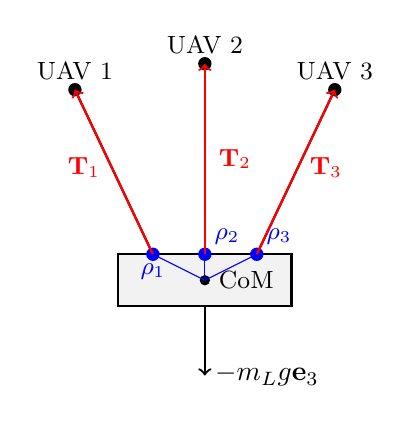
\begin{tikzpicture}[scale=1.1]
  % Payload box
  \draw[thick,fill=gray!10] (-1.0,-0.3) rectangle (1.0,0.3);

  % Centre of mass marker
  \filldraw (0,0) circle (1.5pt);
  \node[right, font=\small] at (0.05,0) {CoM};

  % Gravity
  \draw[->,thick] (0,-0.3) -- (0,-1.1) 
      node[right] {$-m_L g \mathbf{e}_3$};

  % Attachment points on payload surface
  \filldraw[blue] (-0.6,0.3) circle (2pt);
  \filldraw[blue] (0.0,0.3) circle (2pt);
  \filldraw[blue] (0.6,0.3) circle (2pt);

  % UAV 1 - left
  \filldraw (-1.5, 2.2) circle (2pt);
  \node[above, font=\small] at (-1.5,2.2) {UAV 1};
  \draw[thick] (-1.5,2.2) -- (-0.6,0.3);
  \draw[->,red,thick] (-0.6,0.3) -- (-1.5,2.2);
  \node[left, font=\small, red] at (-1.1,1.3) {$\mathbf{T}_1$};
  \draw[->,blue] (0,0) -- (-0.6,0.3) 
      node[below, font=\small, blue] {$\boldsymbol{\rho}_1$};

  % UAV 2 - centre
  \filldraw (0, 2.5) circle (2pt);
  \node[above, font=\small] at (0,2.5) {UAV 2};
  \draw[thick] (0,2.5) -- (0,0.3);
  \draw[->,red,thick] (0,0.3) -- (0,2.5);
  \node[right, font=\small, red] at (0.05,1.4) {$\mathbf{T}_2$};
  \draw[->,blue] (0,0) -- (0,0.3)
      node[above right, font=\small, blue] {$\boldsymbol{\rho}_2$};

  % UAV 3 - right
  \filldraw (1.5, 2.2) circle (2pt);
  \node[above, font=\small] at (1.5,2.2) {UAV 3};
  \draw[thick] (1.5,2.2) -- (0.6,0.3);
  \draw[->,red,thick] (0.6,0.3) -- (1.5,2.2);
  \node[right, font=\small, red] at (1.1,1.3) {$\mathbf{T}_3$};
  \draw[->,blue] (0,0) -- (0.6,0.3)
      node[above right, font=\small, blue] {$\boldsymbol{\rho}_3$};

\end{tikzpicture}
\caption[Multi-UAV payload system]{Multi-UAV payload system: rod $i$ pulls on the payload with tension $\mathbf{T}_i = \lambda_i \mathbf{q}_i$ at the attachment point $\boldsymbol{\rho}_i$, offset from the payload's CoM.}
\label{fig:payload_system}
\end{figure}

Rod $i$ contributes its direction $\mathbf{q}_i$, the angular velocity of that direction $\mathbf{r}_i$
and its first two derivatives, and the tension $\lambda_i$ with its rate:
\begin{equation}
    \mathbf{x} = \big[\, \mathbf{p}_L,\ \mathbf{v}_L,\ \mathbf{q}_L,\ \boldsymbol{\omega}_L,\
    \{\mathbf{q}_i,\ \mathbf{r}_i,\ \dot{\mathbf{r}}_i,\ \ddot{\mathbf{r}}_i,\ \lambda_i,\ \dot{\lambda}_i\}_{i=1}^{N} \,\big]
    \in \mathbb{R}^{13+14N}.
\end{equation}
The inputs are the third derivative of each rod's angular velocity and the second derivative of its
tension, $\mathbf{u} = \{\boldsymbol{\gamma}_i, \eta_i\}_{i=1}^N$, so that the tensions and the rod
directions, and with them the UAV accelerations, are smooth. The dynamics are the payload's
Newton--Euler equations and the rod kinematics:
\begin{align}
    \dot{\mathbf{p}}_L &= \mathbf{v}_L, &
    m_L \dot{\mathbf{v}}_L &= \sum_{i=1}^{N} \lambda_i \mathbf{q}_i - m_L g \mathbf{e}_3 + \mathbf{d},
    \label{eq:plan_trans} \\
    \dot{\mathbf{q}}_L &= \tfrac{1}{2}\, \mathbf{q}_L \otimes \begin{bmatrix} 0 \\ \boldsymbol{\omega}_L \end{bmatrix}, &
    \mathbf{J}_L \dot{\boldsymbol{\omega}}_L &= \sum_{i=1}^{N} \lambda_i\, \boldsymbol{\rho}_i \times R_L^\top \mathbf{q}_i
    - \boldsymbol{\omega}_L \times \mathbf{J}_L \boldsymbol{\omega}_L, \\
    \dot{\mathbf{q}}_i &= \mathbf{r}_i \times \mathbf{q}_i, &
    \dddot{\mathbf{r}}_i &= \boldsymbol{\gamma}_i, \qquad \ddot{\lambda}_i = \eta_i,
\end{align}
where $\mathbf{d}$ is a constant force on the payload, zero in the original formulation and used for
steady-error rejection in Section~\ref{sec:disturbance}. The UAV positions follow from the rod
kinematics,
\begin{equation}
    \mathbf{p}_i = \mathbf{p}_L + R_L \boldsymbol{\rho}_i + l_i \mathbf{q}_i - \boldsymbol{\delta},
    \label{eq:rod_kin}
\end{equation}
with $\boldsymbol{\delta}$ the position of the rod pivot relative to the UAV's
centre ($\boldsymbol{\delta} = -0.04\,\mathbf{e}_3$\,m on the rig). The rod tension couples the system:
it drives the payload in \eqref{eq:plan_trans} and acts, equal and opposite, on UAV $i$.
Differentiating \eqref{eq:rod_kin} twice gives $\ddot{\mathbf{p}}_i$, and the thrust each UAV of mass
$m_q$ must produce is
\begin{equation}
    \mathbf{f}_i = m_q\big(\ddot{\mathbf{p}}_i + g\mathbf{e}_3\big) + \lambda_i \mathbf{q}_i .
    \label{eq:thrust_req}
\end{equation}
The state grows linearly with $N$, which drives the computational scaling noted in \cite{tudelft}.


% controller.tex -- draft of the controller as flown (4 Oct 2026), input from Methodology.tex.
% Notation follows Source/src/model.tex: q_i points from the payload attachment to UAV i and
% T_i = lambda_i q_i. The code (mpc_planner, after Sun et al.) uses s_i = -q_i and t_i = lambda_i.
% Restructured 9 Oct (structure audit): the model moved to model.tex; planner, tracker and steady-error
% rejection are subsections of their own; the result numbers (the box's effect, K's measured values,
% the damping ratio) moved to Section 4.2; the thrust identification procedure moved here from
% hardware.tex; the cost weights moved to Appendix B. Notation: the horizon has N_h nodes over T_h
% (were N and T, which also named the team size and the tension).
% Its references (francis1976internal, pannocchia2003disturbance, pannocchia2007combined,
% maeder2009linear, verschueren2022acados) are in references.bib.

\subsection{Load--cable planner}
\label{sec:controller}

The controller is a two-level cascade of model predictive controllers (Figure~\ref{fig:cascade}).
A centralised planner, based on the load--cable formulation of \cite{tudelft}, plans the motion of
the payload and of every rod over a horizon. Each UAV runs its own tracking MPC, which follows the
planner's reference for that UAV and accounts for the planned rod force. The tracker's output
(collective throttle and three body-rate commands) is sent over the radio link to the flight
controller, whose inner rate loop is not modified. Both levels are solved with acados
\cite{verschueren2022acados} using a real-time iteration (RTI) scheme \cite{diehl2002rti}: one
Gauss--Newton SQP step per tick, warm-started from the previous solution, with the QPs solved by
HPIPM \cite{frison2020hpipm} (partial condensing in the planner, full condensing in the tracker).
Both horizons have $N_h = 20$ nodes over $T_h = 2$\,s.

\begin{figure}[h]
\centering
\begin{tikzpicture}[node distance=1.0cm and 1.3cm, >=Stealth,
    blk/.style={draw, thick, rounded corners=2pt, align=center, minimum height=1.0cm, font=\small},
    lab/.style={font=\scriptsize, align=center}]
  \node[blk, minimum width=3.2cm] (plan) {Load--cable planner\\ \scriptsize 10\,Hz, $N_h=20$, $T_h=2$\,s};
  \node[blk, right=2.0cm of plan, minimum width=2.8cm] (trk) {Tracking MPC $i$\\ \scriptsize 50\,Hz, one per UAV};
  \node[blk, right=1.3cm of trk, minimum width=2.2cm] (fc) {Flight controller\\ \scriptsize rate loop};
  \node[blk, below=1.1cm of trk, minimum width=2.8cm] (sys) {UAVs, rods and payload};
  \node[blk, below=1.1cm of plan, minimum width=3.2cm] (dist) {Payload state, $\mathbf{d}$\\ \scriptsize integral, estimate};
  \draw[->, thick] (plan) -- node[lab, above] {$\mathbf{p}_i, \mathbf{v}_i, \mathbf{a}_i,$\\ $\mathbf{a}_{c,i}, u_{T,i}^{\mathrm{ff}}$} (trk);
  \draw[->, thick] (trk) -- node[lab, above] {$u_T, \boldsymbol{\omega}_{\mathrm{cmd}}$} (fc);
  \draw[->, thick] (fc) |- (sys);
  \draw[->, thick] (sys) -- node[lab, right] {mocap:\\ UAV state} (trk);
  \draw[->, thick] (sys) -- node[lab, below] {mocap:\\ payload pose} (dist);
  \draw[->, thick] (dist) -- node[lab, left] {$\hat{\mathbf{x}}_L, \mathbf{d}$} (plan);
\end{tikzpicture}
\caption[Controller structure]{Controller structure. Motion capture closes both loops; the disturbance term enters the
planner's model.}
\label{fig:cascade}
\end{figure}

The planner works on the model of Section~\ref{sec:model}.

\paragraph{Optimal control problem.} At each planner tick the planner solves
\begin{equation}
\begin{aligned}
    \min_{\mathbf{x}_{0:N_h},\, \mathbf{u}_{0:N_h-1}} \quad & \sum_{k=0}^{N_h-1} \big\| \mathbf{y}(\mathbf{x}_k, \mathbf{u}_k) - \mathbf{y}_k^{\mathrm{ref}} \big\|_{W}^{2}
    + \big\| \mathbf{y}_{N_h}(\mathbf{x}_{N_h}) - \mathbf{y}_{N_h}^{\mathrm{ref}} \big\|_{W_{N_h}}^{2} \\
    \text{s.t.} \quad & \mathbf{x}_{k+1} = \mathbf{F}(\mathbf{x}_k, \mathbf{u}_k; \mathbf{d}), \\
    & C_0 \mathbf{x}_0 = C_0 \hat{\mathbf{x}}(t), \\
    & \lambda_{\min} \le \lambda_{i,k} \le \lambda_{\max}, \quad f_{\min} \le \|\mathbf{f}_{i,k}\| \le f_{\max}, \\
    & |\boldsymbol{\gamma}_{i,k}| \le \gamma_{\max}, \quad |\eta_{i,k}| \le \eta_{\max},
\end{aligned}
\label{eq:plan_ocp}
\end{equation}
with the output
$\mathbf{y} = [\mathbf{p}_L, \mathbf{v}_L, \mathbf{e}_R, \boldsymbol{\omega}_L, \{\mathbf{q}_i\}, \{\lambda_i\}, \{\mathbf{r}_i\}, \mathbf{u}]$,
where $\mathbf{e}_R = 2\,\mathrm{vec}(\mathbf{q}_L^{\mathrm{ref}} \otimes \mathbf{q}_L^{*})$ is the sign-invariant
attitude error. The thrust bounds are softened with slack. $\mathbf{F}$ is the integrated dynamics
over one node of $T_h/N_h = 0.1$\,s.

The initial-condition constraint pins only what motion capture measures directly: the payload pose
and twist, and each rod direction ($C_0$ selects $\mathbf{p}_L, \mathbf{v}_L, \mathbf{q}_L,
\boldsymbol{\omega}_L, \mathbf{q}_i$). The rod rates and their derivatives and the tensions are free
decision variables at node 0, warm-started from the previous solution. Pinning a tension carried over
from the last plan against a measured pose that the UAVs did not quite reach makes node 0 inconsistent.

\paragraph{References.} The payload reference $(\mathbf{p}_L^{\mathrm{ref}}, \mathbf{v}_L^{\mathrm{ref}},
\mathbf{a}_L^{\mathrm{ref}})$ comes from the lift schedule and the trajectory. The rod references are
derived from it by flatness. Holding the payload against gravity, its acceleration and the force
$\mathbf{d}$ needs the rods to support the effective gravity
\begin{equation}
    \mathbf{g}_{\mathrm{eff}} = g\mathbf{e}_3 + \mathbf{a}_{L,xy}^{\mathrm{ref}} - \mathbf{d}/m_L ,
\end{equation}
where $\mathbf{a}_{L,xy}^{\mathrm{ref}}$ is the horizontal part of the reference acceleration (the
trajectories are level),
and the nominal formation (each rod at 45$^\circ$ elevation, tensions $\lambda_i^{0}$ balancing the payload
weight) is rotated so that its vertical axis lies along $\mathbf{g}_{\mathrm{eff}}$, and the tensions are
scaled to $\lambda_i^{\mathrm{ref}} = \lambda_i^{0}\, \|\mathbf{g}_{\mathrm{eff}}\| / g$.

The weights are listed in Table~\ref{tab:weights} (Appendix~\ref{sec:app_params}). The weight on the rod
directions holds the formation's shape, and the weight on the rod rates damps rod swing.

\paragraph{Output to the trackers.} From the solved horizon the planner sends each tracker its
reference position, velocity and acceleration from \eqref{eq:rod_kin}, the planned cable acceleration
$\mathbf{a}_{c,i} = -\lambda_i \mathbf{q}_i / m_q$ at every node, and a throttle feedforward from
$\|\mathbf{f}_i\|$ in \eqref{eq:thrust_req}. The reference is the whole horizon, not a single
set-point, and the tracker interpolates it at its own rate, so a late or skipped planner tick does not
leave it without a reference.

\subsection{UAV tracking MPC and thrust map}
\label{sec:tracker}

Each UAV $i$ runs a tracking MPC on a 17-state model, in which the four stick channels sent to the
flight controller are themselves states and their rates of change are the inputs:
\begin{equation}
    \mathbf{x}_i = [\mathbf{p},\ \mathbf{q},\ \mathbf{v},\ \boldsymbol{\omega},\ \mathbf{c}], \qquad
    \mathbf{c} = [c_\phi, c_\theta, u_T, c_\psi], \qquad \mathbf{u}_i = \dot{\mathbf{c}},
\end{equation}
with
\begin{align}
    \dot{\mathbf{p}} &= \mathbf{v}, &
    \dot{\mathbf{q}} &= \tfrac{1}{2}\, \Omega(\boldsymbol{\omega})\, \mathbf{q}, \\
    \dot{\mathbf{v}} &= R(\mathbf{q})\, k_T u_T \mathbf{e}_3 - g\mathbf{e}_3 - c_z v_z \mathbf{e}_3 + \mathbf{a}_{c,i}, &
    \dot{\boldsymbol{\omega}} &= \frac{1}{\tau_\omega}\big(\boldsymbol{\omega}_{\mathrm{cmd}}(\mathbf{c}) - \boldsymbol{\omega}\big),
    \label{eq:trk_model}
\end{align}
where $\boldsymbol{\omega}_{\mathrm{cmd}}(\mathbf{c})$ is the flight controller's rate curve applied to the
roll, pitch and yaw sticks, and $\tau_\omega$ the time constant of its rate loop. Thrust is modelled
as affine in throttle, identified on the rig: the throttle sent is $u_T + u_0(V)$, with the offset
$u_0(V) = u_0 + \kappa (V_{\mathrm{ref}} - V)$ correcting for the battery voltage $V$ and $k_T$ the gain
above it. The planned cable acceleration $\mathbf{a}_{c,i}$ enters the model as a known, time-varying
parameter along the horizon, so the tracker anticipates the rod's pull instead of reacting to it.
The planned pull is only as good as the planner's model of the rods. On the rig the rods flew at about
60$^\circ$ from horizontal where the plan assumed 45$^\circ$, so each tracker now measures the pull and uses the
plan only for its shape along the horizon: the measured pull is the UAV's acceleration from motion capture
(the least-squares slope of its velocity over 80\,ms, low-pass filtered at 50\,ms) minus the modelled thrust,
gravity and drag, with the thrust passed through the same filter so that a throttle change does not read as
a change of pull. The horizon's planned pull is shifted by the difference between the measured and the
planned pull at its first node, and the result is capped at 12\,m/s$^2$. The planner plans the rods at
60$^\circ$ to match. Section~\ref{sec:res_rig_integral} gives its effect on the rig.

The tracker solves, every 20\,ms,
\begin{equation}
\begin{aligned}
    \min \quad & \sum_{k=0}^{N_h-1} \big\| \mathbf{h}(\mathbf{x}_k, \mathbf{u}_k) - \mathbf{h}_k^{\mathrm{ref}} \big\|_{Q}^{2} + \big\| \mathbf{h}_{N_h}(\mathbf{x}_{N_h}) - \mathbf{h}_{N_h}^{\mathrm{ref}} \big\|_{Q_{N_h}}^{2} \\
    \text{s.t.} \quad & \mathbf{x}_{k+1} = \mathbf{F}_i(\mathbf{x}_k, \mathbf{u}_k; \mathbf{a}_{c,i,k}), \qquad \mathbf{x}_0 = \hat{\mathbf{x}}_i(t), \\
    & 0.05 \le u_{T,k} \le u_{T,\max}, \quad |c_{\phi,k}|, |c_{\theta,k}|, |c_{\psi,k}| \le 1, \quad |\mathbf{u}_k| \le \overline{\mathbf{u}},
\end{aligned}
\label{eq:trk_ocp}
\end{equation}
with $\mathbf{h} = [\mathbf{p}, \mathbf{v}, \boldsymbol{\omega}, \mathbf{c}, \mathbf{u}, \mathbf{e}_R]$, the
attitude reference being the direction of the planned thrust \eqref{eq:thrust_req}. The stick states
are normalised to $[-1, 1]$, and $\overline{\mathbf{u}}$ limits how fast each may change (throttle
0.5\,s$^{-1}$). Only the first command of each solution is sent.

\paragraph{Initial condition.} Node 0 equals the measured state, $\mathbf{x}_0 = \hat{\mathbf{x}}_i(t)$,
which is the standard formulation. The stick states in $\hat{\mathbf{x}}_i$ are the commands actually
sent, not the last solution, so the model starts from where the actuators are. An earlier version
relaxed this to the box $\hat{\mathbf{x}}_i(1-\epsilon) \le \mathbf{x}_0 \le \hat{\mathbf{x}}_i(1+\epsilon)$
with $\epsilon = 0.025$; Section~\ref{sec:res_ic} shows its effect.

\paragraph{Thrust identification.} A proportional map with one gain, identified at hover, did not
hold across loads and battery states. The map was therefore identified on the rig: each UAV hovered
free with hung masses of 0, 98 and 196\,g over battery voltages of 22.7--24.6\,V, and the throttle it
needed was fitted against the mass it carried and the voltage. The fit and $k_T$ are in
Section~\ref{sec:thrust_id}.

\subsection{Steady-error rejection}
\label{sec:disturbance}

Any error that remains constant, from a model mismatch or an external force, is represented by the
constant force $\mathbf{d}$ on the payload in \eqref{eq:plan_trans}. $\mathbf{d}$ is a lumped disturbance:
for an external force (wind, a push, an unmodelled object in the basket) it is that force; for an
internal error (a thrust-map error, the rods' mass) it is the force that would have the same effect on
the payload, which need not exist physically. In the offset-free MPC literature this is an input
disturbance model \cite{pannocchia2003disturbance, maeder2009linear}.

\paragraph{Integral action through the model.} $\mathbf{d}$ is formed from the integral of the payload's
position error $\mathbf{e}_k = \mathbf{p}_L^{\mathrm{ref}} - \mathbf{p}_L$, updated at each planner tick
$k$ (period $T_s = 0.1$\,s):
\begin{equation}
    \mathbf{b}_{k+1} = \mathrm{sat}_{\bar{b}}\!\big(\mathbf{b}_k + k_i T_s\, G_k\, \mathbf{e}_k\big), \qquad
    \mathbf{d}_k = -K \mathbf{b}_k, \qquad K = \mathrm{diag}(K_{xy}, K_{xy}, K_z).
    \label{eq:lumped_int}
\end{equation}
Here $\mathrm{sat}_{\bar{b}}$ bounds each component to $\pm\bar{b}$, and $G_k = \mathrm{diag}(g_{xy}, g_{xy}, g_z)
\in \{0,1\}^3$ is a gate. The gate integrates only in steady, taut flight: lift complete, not
descending or landing, every rod taut, a fresh pose, the payload slow ($<0.05$\,m/s) and the miss
under 0.25\,m. The vertical component also integrates through a slow level orbit. The horizontal
components require a stationary reference, so a value learned in hover is held through a trajectory. A low payload ($e_z > 0$) makes $d_z$ negative: the planner then believes the payload is
heavier and plans more rod tension. Once the payload rests on the floor at landing, $\mathbf{d}$ is
set to zero.

$K$ converts the integral from metres to newtons. It is set to the closed-loop stiffness of the
cascade to a force on the payload, measured by applying a known force and recording the steady
displacement (Section~\ref{sec:res_force}). With this choice the integral's loop gain is
$k_i$, the same as for the equivalent reference-shift form below.

\paragraph{Where $\mathbf{d}$ enters.} $\mathbf{d}_k$ is a parameter of the planner's problem, constant
over the horizon and refreshed at every tick. It enters the payload's translational dynamics
\eqref{eq:plan_trans}, so the plan predicts the payload's motion with the force included and chooses
tensions and UAV positions that counter it. It also enters the reference formation through the
effective gravity $\mathbf{g}_{\mathrm{eff}}$ of the references above, so the formation the cost draws
the solution towards is already tilted and tensioned to balance $\mathbf{d}$, and the cost does not
oppose the force balance.

\paragraph{Zero steady-state error.} Suppose the closed loop converges to an equilibrium at which the
gate is open ($G = I$) and no component of $\mathbf{b}$ is saturated. Then $\mathbf{b}_{k+1} = \mathbf{b}_k$
in \eqref{eq:lumped_int} gives $k_i T_s \mathbf{e} = \mathbf{0}$, so $\mathbf{e} = \mathbf{0}$, whatever
the constant cause. This is the internal model principle \cite{francis1976internal}: a constant
disturbance is rejected because the controller contains a model of a constant, the integrator. The
statement assumes stability; it does not give it. Approximating the cascade's response to $\mathbf{d}$
by a first-order lag with time constant $\tau$, each axis becomes
\begin{equation}
    \tau s^2 + s + k_i = 0, \qquad \zeta = \frac{1}{2\sqrt{k_i \tau}},
\end{equation}
so a faster integral costs damping (Section~\ref{sec:res_force} gives $\zeta$ for the measured $\tau$). Time delays through the planner and the radio link reduce the margin further.

\paragraph{What the integral learns.} Let an unmodelled constant force $\mathbf{F}$ act on the payload,
let $K_c$ be the cascade's actual stiffness to a force on the payload, and treat the cascade as
quasi-static (fast compared with the integral). The plan cancels the force it believes in, $\mathbf{d}$,
so the payload settles displaced by $K_c^{-1}(\mathbf{F} - \mathbf{d})$ and
$\mathbf{e} = -K_c^{-1}(\mathbf{F} - \mathbf{d}) = -K_c^{-1}(\mathbf{F} + K\mathbf{b})$. In continuous time
\eqref{eq:lumped_int} becomes
\begin{equation}
    \dot{\mathbf{b}} = k_i\,\mathbf{e} = -k_i K_c^{-1}\big(K\mathbf{b} + \mathbf{F}\big)
    \quad\Rightarrow\quad \mathbf{b} \to -K^{-1}\mathbf{F}, \qquad \mathbf{d} \to \mathbf{F},
\end{equation}
a first-order convergence at the rate $k_i K K_c^{-1}$ on each axis, with time constant $1/k_i = 2.5$\,s when
$K = K_c$. The believed force converges to the applied one whatever $K$ is: $K$ sets only the speed,
and too large a $K$ costs damping as too large a $k_i$ does. When the force is removed, $\mathbf{b}$
still holds $-K^{-1}\mathbf{F}$, so the payload overshoots by $K_c^{-1}\mathbf{F}$, the displacement the
force caused at onset, and the overshoot decays at the same rate. Section~\ref{sec:res_force} measures both: the
learned force against the applied one, and the overshoot on release.

\paragraph{Reference-shift form.} An earlier version added the height integral to the payload's height
target instead, $z_L^{\mathrm{ref}} \leftarrow z_L^{\mathrm{ref}} + b_z$. Both forms are integral action and
reach the same steady state. In the offset-free MPC literature they correspond to output and input
disturbance models, which differ in transient behaviour, not in the steady state
\cite{pannocchia2007combined}. The model form keeps the target fixed. Its plan predicts a payload
held at the target, which is what happens. The reference-shift form plans a move towards the shifted
target that never comes. The model form also extends to the horizontal axes.

The model form is the default, on the rig as well as in simulation. Where it is not used, the
reference-shift form flies instead, on the height only: wherever the fleet can attach or detach
mid-flight, since the problem is resized with the integral in it, and wherever the integral is
switched off. The rig flights so far used the reference-shift form, as a bounded safety net with
$k_i = 0.4$\,s$^{-1}$.
% STATUS 5 Oct 2026: int_mode auto (model where allowed, else reference): reference with kt_trim on,
% a resizing fleet, z_ki 0, offset_free on or dist_est ring/full (bringup real_mode.planner_options).

\paragraph{Bound.} $\bar{b} = 0.3$\,m bounds the force the integral can supply to $K\bar{b}$ (2.1\,N
vertically), enough for an unmodelled 0.1\,kg object. The bound is a safety measure: a larger error is
a fault, not a disturbance. A warning is raised at 70\,\% of it, so that a fault is reported rather than
silently covered.

\paragraph{Limits.} The integral corrects forces on the payload, not moments: a constant moment, such as
one UAV's thrust-map error, still tilts the payload. A miss larger than the gate is never integrated,
so an error that large stays (Section~\ref{sec:sim_robustness}). The integral is also slow
($1/k_i = 2.5$\,s): it removes constant and slowly varying forces, not impacts or gusts, which only a
force measured on board each UAV could counter quickly.

\paragraph{Alternatives.} Five other ways to remove a steady error were built and flown on the same
cases as the integral (Section~\ref{sec:sim_methods}):
\begin{description}
    \item[Force balance] estimates a constant force on the ring and one shared by the UAVs from the
    measured motion and the delivered thrust, and gives them to the planner's model
    \cite{muske2002disturbance}.
    \item[Offset-free observer] estimates the force from the planner's own prediction error, as in
    offset-free MPC \cite{pannocchia2003disturbance}.
    \item[Measured cable force] each tracker takes its rod's force from its measured acceleration and
    delivered thrust, the ground-side counterpart of the compensation from inertial measurements of
    \cite{tudelft}.
    \item[Thrust-gain trim] a per-UAV estimate of the throttle-to-acceleration gain, from the UAV's own
    measured acceleration and its static share of the rod force.
    \item[Rod mass in the planner] the rods' mass added to the planner's model.
\end{description}

% Under evaluation (sim only): option A, a direct estimate of d from the measured motion and the
% delivered thrust. Per sample, least squares over the tensions, d_L and a force d_D shared by the
% UAVs, from
%   UAV i:    m_q a_i = f_i R_i e3 - m_q g e3 - lambda_i q_i + d_D
%   payload:  m_L a_L = sum_i lambda_i q_i - m_L g e3 + d_L
% filtered by two first-order stages. In the code it is not yet combined with eq:lumped_int.



% takeoff_landing.tex -- Methodology: takeoff from the floor, lift and landing (draft 4 Oct 2026).
% Code: mpc_planner/creep_controller.py (arc creep, hand-over latch), planner_node.py (pretension,
% breakaway, ff_cap_release_s, lift ramp, LAND, TouchdownDetector), bringup/config/*.yaml.
% Evidence: 23 Sep rig non-lift (start_taut), 30 Sep rig review, R0817/R0818, R0834-R0839 (B2),
% R0807-R0816 (hand-over angle in the twin), RIG-1001-* (hand-over and rods on the rig).
% Condensed 12 Oct 2026 to the plan's half page; the detail is Appendix C "Floor start and landing in detail".
% Restructured 9 Oct (structure audit): the outcomes (the hand-over angle flown, fig:flight) moved to
% Section 4.1.

\subsubsection{Takeoff, lift and landing}
\label{sec:takeoff}

The planner assumes taut rods, but every flight starts and ends with the ring on the floor and the rods slack or
flat, where the UAVs sit about 0.7\,m from the ring's centre, outside the cone the planner's references put them
on; started from rest, the planner pulled the UAVs inwards over the ring instead of lifting it, the cause of the
first failed lifts on the rig. Four steps take a flight from the floor into the regime the planner models, and three
measures take it back; Appendix~\ref{sec:app_floor} gives each with its numbers and the failure it answers.
\begin{itemize}
    \item \textbf{Rod sweep.} On TAKEOFF each UAV is anchored where it rests and its rod is swept about its own
    attachment point from its measured elevation to the planned one (60$^\circ$ since 7 October), the UAV's
    reference riding the far end of the rod, so that the rod stays straight and the UAV never crosses over the
    ring. The planner takes over once every rod has held within 8$^\circ$ of the planned elevation for 1\,s, and
    measures each rod's length from motion capture at that hand-over for its model and its tautness gate.
    \item \textbf{Pretension and breakaway.} Every UAV's share of the planned pull then rises together from zero
    over 3\,s with the ring's height target at its resting height; a step here launched the ring and released two
    magnets on the rig. When the ring rises 1\,cm or faster than 0.03\,m/s it has broken free, and the fraction of
    the planned pull reached at that moment is frozen as a cap on the trackers' feedforward, released back to the
    full pull over 2\,s once the lift starts.
    \item \textbf{Lift.} The height target ramps to the target height at 0.1\,m/s, eased in and out, and the
    trajectory starts when the ramp completes.
    \item \textbf{Landing.} On LAND the ring's height target descends at 0.2\,m/s with the formation unchanged
    until the ring rests. A rigid rod then pushes a UAV descending straight down outward as the rod lengthens
    horizontally, which tipped UAVs over in the twin, so each UAV's reference unwinds along its rod's circle about
    the grounded attachment point before it descends (twin only: the rig's tethers go slack and it lands straight
    down); the planner blends each UAV's thrust and rod feedforward to plain hover over 1\,s instead of dropping
    the rod term at touchdown; and a UAV back at its resting height with the ring down idles armed until the fleet
    disarms, so that a UAV that lands first does not track a reference below the floor. Touchdown is declared when
    the UAVs stop following the descending reference for 1\,s after at least 5\,cm of descent, and the fleet
    manager disarms the fleet.
\end{itemize}


% reconfiguration.tex -- Methodology: reconfiguration (detach and attach). Draft 4 Oct 2026.
% Code: dissipative_planner/dissipative_node.py (_detach_ocp, _attach_ocp, _capture_weld_rho,
% partner hand-off), dissipative_planner/approach.py, drone_magnet (magnet_attachment_manager,
% elrs_mux, handover_policy, attach_target_publisher), bringup/bringup/graph_attach.py.
% Evidence: CURRENT_STATE 4.1, 4.2, 4.11; notes 2026-09-24_detach_land_fix, 2026-09-25_attach_ocp,
% 2026-09-27_m1_rejoin, 2026-09-27_m1_full, 2026-09-27_m2_handover.

\subsection{Reconfiguration by OCP resize}
\label{sec:reconfig}

A reconfiguration changes the number of UAVs carrying the payload in the air. In the final design both
directions are handled the same way: the planner switches to a solver for the new team size and carries
on. This subsection describes the detach, the attach, and the design each replaced.

\subsubsection{Detach}

On DETACH the departing UAV's magnet releases the rod at the payload end, the UAV flies away with its
rod, and the planner continues with the survivors. Two approaches were built and compared.

\paragraph{OCP resize.} The planner keeps flying the payload and re-solves for the smaller fleet, which
two properties of the formulation make possible.
\begin{itemize}
    \item The attachment points $\boldsymbol{\rho}_i$ and rod lengths $l_i$ are runtime parameters of
    the model, not constants compiled into the solver. Only the fleet size fixes the problem
    dimensions, so one solver per fleet size, built in advance, covers any attachment layout.
    \item The survivors keep their own attachment points. The rods stay where they were on the ring,
    so three survivors of a four-UAV ring sit, for example, at 0, 90 and 180$^\circ$, not at an even
    0, 120 and 240$^\circ$. Handing the planner an even ring instead makes its moment balance wrong by
    construction.
    \redo{the hand-back to an even ring after a detach from four UAVs (the survivors at 0, 90 and 180$^\circ$, the planner told 0, 120 and 240$^\circ$): payload tilt.}
% --- original text, flown before the rig twin; kept to refill this place:
%     0, 120 and 240$^\circ$. Handing the planner an even ring instead makes its moment balance wrong by
%     construction; in an early test this tipped the payload by 62$^\circ$.
\end{itemize}
At the detach the planner swaps to the solver for $N-1$ UAVs, sets the survivors' attachment points and
rod lengths, and warm-starts the new problem from the measured state. The tensions and rod directions are
free at node~0, so the first solve redistributes the load, with no separate hand-off phase. A detach is
refused if it would leave fewer than three UAVs, and during LAND.

\paragraph{Network hand-off.} The alternative, closer to the decentralised literature
\cite{quan2025swarm}, hands the payload to the dissipative network of Section~\ref{sec:dissipative} on the
detach; the network holds it while it redistributes the load between the survivors, then hands back to a
planner built for $N-1$. Section~\ref{sec:sim_detach} compares the two; the OCP resize is the detach used
in the rest of this work.
% --- original text, flown before the rig twin; kept to refill this place:
% then hands back to a planner built for $N-1$. In simulation the OCP resize won this comparison
% clearly (Section~\ref{sec:sim_detach}), and it is the detach used in the rest of this work.

% Departed landing (pressed to its rest, disarmed alone): twin 9 Oct, card 2026-10-09_departed_disarm_alone;
% the default once the LAND re-fly's reviewer passes it; rig W4/W5 on 14 Oct.
\paragraph{The departing UAV.} After the release, switched on the rig by the same DETACH command on the
UAV's magnet channel, the departing UAV steps 0.5\,m out radially at its height, clear of the ring and the
survivors, and lands on its own while the survivors carry on. Its height reference is pressed below its
own resting height until it gets there, and it is then disarmed alone, without waiting for the fleet
(Section~\ref{sec:res_detach_rig}).

\paragraph{Layout.} Whether the payload can still hang level after a detach depends on the geometry, not
on the controller: its centre of mass must stay inside the polygon of the surviving attachment points.
Removing one UAV from an even ring of $N$ leaves a largest angular gap of $4\pi/N$, which keeps the centre
inside only for $N \ge 5$; $N = 4$ sits exactly on the boundary. The four-UAV flights therefore use the
plates at 30, 90, 150 and 270$^\circ$, and detaching the UAV at 90$^\circ$ leaves an even triangle under
which the ring hangs level. With an uneven layout the planner's nominal tensions come from a moment
balance at the actual attachment points, so they are unequal and the payload's reference stays level.

\paragraph{Landing after a detach.} Touchdown is judged on the survivors only, so a departed UAV still
descending elsewhere does not hold their references down; a departed UAV is judged down at its own
resting height, and the fleet is declared landed only when it is down too. The cable feedforward is
switched off once the payload rests, because its sideways component pushes a grounded survivor across
the floor.
% --- original text, flown before the rig twin; kept to refill this place:
% declared landed only when they are down too. The cable feedforward is switched off once the payload
% rests, because its sideways component pushed a grounded survivor across the floor until it tipped
% in an early version.

\subsubsection{Attach}

On ATTACH a free UAV (the newcomer) approaches its attachment point, its magnet welds to a plate on the
ring, and the planner folds it into the team. The approach controller, the approach UAV and its magnet
are the collaborating student's; this work takes over at the weld.
% TODO: cite the collaborator's thesis or report once available.

\paragraph{Sequence.}
\begin{enumerate}
    \item \textbf{Target hold.} ATTACH freezes the payload's horizontal reference, or keeps it on its
    trajectory when the payload is moving, shifted onto the measured payload position, so the newcomer
    approaches where the payload actually is.
    \item \textbf{Approach.} The newcomer flies to a point above its plate and descends onto it, flown by
    the collaborator's approach controller or by its own tracker on an approach profile from this work.
    The payload may keep moving, at up to 0.2\,m/s.
    \redo{a weld onto a payload moving at 0.4\,m/s against 0.2\,m/s (the limit on the payload's speed during the approach).}
% --- original text, flown before the rig twin; kept to refill this place:
%     approach profile from this work. The payload may keep moving, at up to 0.2\,m/s; at 0.4\,m/s the
%     weld flipped the payload in simulation.
    \item \textbf{Weld.} A magnet manager welds when the magnet tip is within 8\,cm of the plate point,
    computed from the payload's measured pose, and the relative speed is under 0.05\,m/s, both for 0.15\,s.
    \item \textbf{Authority hand-over.} Until the weld, a multiplexer forwards the approach controller's
    commands to the newcomer's radio; after it, the multiplexer switches to this work's tracker, only on a
    command that is armed and above idle throttle, and latches. An abort latches the mux to a disarmed idle
    command until it is restarted.
    \redo{the authority hand-over at the weld with the mux switching on an armed but idle stream, against the armed-and-above-idle rule: whether the newcomer's motors cut at the weld.}
% --- original text, flown before the rig twin; kept to refill this place:
%     tracker, but only on a command that is armed and above idle throttle. A mux that handed authority
%     to an armed but idle stream cut the newcomer's motors at every weld in early tests. The switch is
%     latched. An abort latches the mux to a disarmed idle command until it is restarted.
    \item \textbf{Fold-in.} The planner records the weld point in the payload frame and switches to
    the solver for $N+1$ UAVs, with the newcomer's tension starting at 0.1\,N and every UAV's tension
    blended to the balanced solution for the new geometry.
    \redo{the fold-in with the newcomer's tension starting at 1\,N against 0.1\,N: payload tilt at the weld.}
% --- original text, flown before the rig twin; kept to refill this place:
%     blended to the balanced solution for the new geometry. A newcomer started at 1\,N of tension
%     pulled the payload with a lever about the incumbents' cable apex and tilted it at the weld.
    \item \textbf{Resume.} The trajectory continues with $N+1$ UAVs.
\end{enumerate}

\paragraph{Replaced design: network attach.} Until mid-September the attach handed the payload to the
dissipative network at the weld: the newcomer was welded as a central lifter and handed out to its ring
slot over 8--12\,s, with the incumbents' tensions blended over the same ramp
(compared in Section~\ref{sec:sim_attach}).
% --- original text, flown before the rig twin; kept to refill this place:
% its ring slot over 8--12\,s, with the incumbents' tensions blended over the same ramp. This flew the
% demonstration of Figure~\ref{fig:attach} on the earlier, lighter ring. On the 0.86\,kg ring the
% network capsized the payload within about 8\,s of every weld in simulation, while the OCP resize held
% the same weld at about 10$^\circ$ (Section~\ref{sec:sim_attach}).

\paragraph{The rejoin mission.} The full mission of Figure~\ref{fig:mission_profile} is assembled with the
collaborator's mission planner. Four UAVs carry the ring around the orbit; one detaches by OCP resize, flies
the collaborator's mission (picking up an object with its magnet and dropping it into the ring), is handed
back at its attach-ready point, approaches, welds and is folded back in by OCP resize, and the fleet lands.
In a ground-start variant the collaborator's controller joins four UAVs to the ring on the floor and hands
them to this work's planner, which lifts and carries it.


% authority.tex -- Methodology 3.5: authority and safety as runtime assurance (drafted 12 Oct 2026 from the thesis
% plan of 11 Oct). The safety paragraph moved here from system_overview.tex (its label sec:safety comes with it);
% fig:owners (F5) replaces the old nodes and cascade figures. The rig switch states in brackets follow plan D6 and
% the M1 plan's D6(a)/(b): they are set per lab day and are not results.

\subsection{Authority and safety}
\label{sec:safety}

Every UAV in the air has exactly one controller sending it commands at every instant, and every phase has a way
down that ends with the UAV disarmed on the floor. Figure~\ref{fig:owners} shows the cascade and who owns what.
The planner owns the ring: it plans the ring's motion and every rod, and hands each carrier's share to that
carrier's tracker. A tracker owns its UAV's radio link; nothing else writes to it. A UAV that is not on the ring
is owned either by its own tracker (a freed carrier landing by itself, a newcomer being taken back) or by the
collaborator's controller (the newcomer through its pickup, transit, drop and descent to contact), and the
multiplexer in front of the newcomer's radio is the one place where ownership changes hands: it forwards the
collaborator's commands until the attach is confirmed, switches to this work's tracker on that tick, and latches.
Below the trackers each flight controller closes only its body-rate loop and arms, disarms and switches its magnet
on channels the tracker sets; the operator holds a disarm button that overrides everything.

\begin{figure}[htbp]
\centering
\begin{tikzpicture}[>=Stealth, font=\small,
    blk/.style={draw, thick, rounded corners=2pt, align=center, minimum height=0.85cm, font=\small},
    ours/.style={blk, fill=blue!6, draw=blue!50!black},
    his/.style={blk, fill=orange!10, draw=orange!60!black},
    fc/.style={blk, fill=gray!12, draw=gray!60},
    lab/.style={font=\scriptsize, align=center}]
  \node[blk]  (op)   at (5.6,1.7)   {Operator\\ \scriptsize disarm button};
  \node[ours] (fm)   at (5.6,0)     {Fleet manager\\ \scriptsize phases, faults, LAND};
  \node[ours] (plan) at (0,0)       {Load--rod planner\\ \scriptsize 10\,Hz; owns the ring};
  \node[ours] (trk)  at (0,-2.5)    {Tracker $i$ (carrier)\\ \scriptsize 50\,Hz; owns UAV $i$};
  \node[ours] (trkn) at (5.6,-2.5)  {Tracker (newcomer)\\ \scriptsize from the attach, or take-back};
  \node[his]  (tej)  at (11.3,-2.5) {Collaborator's controller\\ \scriptsize pickup, transit, drop,\\ \scriptsize descent to contact, lift};
  \node[ours] (mux)  at (5.6,-4.6)  {Mux\\ \scriptsize one owner, latched};
  \node[fc]   (bf)   at (0,-4.6)    {Flight controller $i$\\ \scriptsize Betaflight rate loop, magnet};
  \node[fc]   (bfn)  at (5.6,-6.3)  {Flight controller (newcomer)\\ \scriptsize Betaflight rate loop, magnet};
  \draw[->, thick] (op) -- node[lab, right] {commands} (fm);
  \draw[->, thick] (fm) -- node[lab, above] {phase} (plan);
  \draw[->, thick] (plan) -- node[lab, left] {reference,\\ rod pull} (trk);
  \draw[->, thick] (plan.south east) -- node[lab, sloped, above, pos=0.55] {once folded in} (trkn.north west);
  \draw[->, thick] (trk) -- node[lab, left] {throttle, rates,\\ arm, magnet} (bf);
  \draw[->, thick] (trkn) -- (mux);
  \draw[->, thick] (tej.south) -- ++(0,-1.25) -- node[lab, above] {until the attach} (mux.east);
  \draw[->, thick] (mux) -- node[lab, right] {one command stream} (bfn);
  \draw[->, thick, dashed] (trk) -- node[lab, above] {fault} (trkn);
  \draw[->, thick, dashed] (fm) -- node[lab, right] {LAND, drop, disarm} (trkn);
  \draw[->, thick, dashed] (fm.north west) -- ++(0,0.5) -| node[lab, pos=0.25, above] {arm, disarm, LAND} ([xshift=-0.5cm]plan.north west) |- (trk.west);
  \draw[<->, thick, dotted] (fm.east) -| node[lab, pos=0.25, above] {attach confirmed, give-up} (tej.north);
\end{tikzpicture}
\caption[The cascade and its owners]{The cascade and its owners. Blue: this work; orange: the collaborator's
controller; grey: the unmodified flight controllers. The planner owns the ring and the carriers' references; each
tracker owns one UAV's radio link; the newcomer's link is owned by the collaborator's controller until the attach
is confirmed and by this work's tracker from that tick, through a multiplexer that latches. Dashed: faults and the
fleet manager's commands; dotted: the confirmation and the give-up exchanged with the collaborator's stack. The
operator's disarm overrides everything.}
\label{fig:owners}
\end{figure}

\paragraph{The envelope and the fleet disarm.} Every tracker checks its own UAV against a flight envelope (UAV tilt
and ring tilt both 60$^\circ$, speed 3\,m/s) and checks that its motion-capture pose (0.25\,s) and the planner's
reference (1\,s) are fresh. A violation on a carrier disarms the whole fleet, not the one UAV: a single UAV losing
thrust on a shared rigid payload drags the others with it, and three UAVs cannot hold a ring hung for four. There
is no geofence. The argument for a fleet disarm rather than a geofenced recovery is the lab itself: the ring flies
at 1\,m inside a 6\,$\times$\,6\,$\times$\,4\,m cage, so a falling ring is a short fall onto a padded floor, where an
armed UAV flying on a wrong reference is not. The exceptions are UAVs that are not on the ring. A fault on a
newcomer that is not yet attached disarms the newcomer alone and lands the fleet, and a UAV that has left the ring
is pushed down to its own resting height and disarmed alone (Section~\ref{sec:reconfig}). LAND lands every UAV,
whatever it is doing. On the rig each UAV must confirm that its flight controller is armed before the fleet takes
off, and a UAV that disarms between ARM and TAKEOFF grounds the fleet, since three UAVs lifting a ring sized for
four would drag it.

\paragraph{The fall-backs, as runtime assurance.} The planner and the admission chain are the high-performance
controllers of a Simplex-style arrangement (Section~\ref{sec:lit_switching}); the fall-backs are simple, each has
its own monitor, and each ends with every UAV owned and down.
\begin{itemize}
    \item \textbf{Take-back.} A newcomer whose contact proves nothing, or whose owner gives up, is taken over by this
    work's tracker, moved clear of the ring and landed by itself (Section~\ref{sec:reconfig}).
    \item \textbf{Tilt cut.} A newcomer whose tilt passes its limit while it is not carrying the ring has its motors
    cut, so that a UAV caught on the rim or on a rod does not drag the ring: [injection to disarm about 0.26\,s in
    the twin; the rig value and the false-cut count over the rig bags, Section~\ref{sec:sim_attach}].
    \item \textbf{LAND for every UAV.} LAND lands the carriers with the ring, a freed carrier where it is, and a
    newcomer wherever it is in its mission, each on its own path down.
    \item \textbf{Landing the fleet on a newcomer fault.} A fault on an unattached newcomer disarms it alone and
    lands the carriers at once, where the earlier rule disarmed all four in the air.
    \item \textbf{Dropping the ring.} A second loss, or a ring tilt over 30$^\circ$, releases every magnet and lands
    every UAV: 30$^\circ$ is where the controller gives up a ring it can no longer hold level, not a value to design
    to (Section~\ref{sec:metrics}).
    \item \textbf{The freed UAV disarmed alone.} A carrier that has left the ring lands by itself and is disarmed at
    its rest without waiting for the fleet, so that the fleet's disarm at the end of a landing never drops it.
\end{itemize}

\paragraph{What is tested where.} ``A tested way down in every phase'' holds in the twin, where every fall-back
above has been flown from the phase it guards (Section~\ref{sec:sim_attach}). On the rig it holds only for the exits
flown there, and the rig switches are set per lab day: [the newcomer's warm tracker through a fault is a candidate
for the 21--22 October launch after its reviewer; the tilt cut and the flight controller's own disarm-to-land stay
off until 28--29 October, so that until then a take-back that sticks ends in a disarm from height; the model
integral through a resize and the freed UAV disarmed alone fly on 14 October]. Redistribution after a release has
flown on the rig; the policy for a true fault on a carrier stays the fleet stop and the drop rule. The
fault-coverage matrix, one row per fault and phase and one column per code tree, is [Appendix~\ref{sec:app_tests},
filled with the results].


\subsection{Method and metrics}
\label{sec:experiments}

Every result is flown against a named baseline, in the rig twin first and on the rig after it, under a rule
written before the runs. The parameters of the twin and of the rig are listed in Appendix~\ref{sec:app_params}.

% simulation.tex -- Methodology: simulation and verification (draft 4 Oct 2026).
% Sources: simulation_assets/ (generate_rigid_world.py, rig-twin worlds), simulation_communication
% (sim Betaflight bridges, rate_pid, imu_world), tools/sil/ (plant, lockstep), tools/run_experiment.py,
% results/registry.csv (832 rows on 4 Oct; run folders R0001-R0986 since 5 Aug), CURRENT_STATE 10.
% Counts: 667 unit tests in this work's packages and tools (4 Oct), excluding the collaborator's.
% Restructured 9 Oct (structure audit): now part of the experimental method; the list of simulator
% artefacts moved to the discussion (Section 4.6), the void rule stays; the SIL bench is defined here;
% the hardware test ladder moved here from hardware.tex.

\subsubsection{Rig twin and experiment runner}
\label{sec:simulation}

Every controller change is tested in simulation before it reaches the rig. The same launch files
and controller code run in simulation and on the rig.

\paragraph{Gazebo rig twin.} The physics simulator is Gazebo \cite{koenig2004gazebo}, connected to
ROS~2 \cite{macenski2022ros2} through bridges. The worlds are generated by a script from the lab's
measured geometry: the 0.86\,kg ring with its twelve plates, UAVs of 0.55\,kg, rods of 0.55\,m and
0.075\,kg with ball joints at both ends, pivoting 4\,cm below each UAV's centre. Each flight starts
with the ring on the floor. A flight controller emulator stands in for Betaflight. It maps the
throttle to rotor speed so that thrust follows the rig's identified affine map, with each UAV's own
offset and a battery that sags under load. It closes a proportional--integral rate loop on the
simulated gyro. A motion-capture emulator publishes the simulated poses on the rig's topics at
120\,Hz.

Wall-clock watchdogs fire when the simulation runs slower than real time, which it does (about 0.3
of real time with the full stack on the laptop); such runs are voided and flown again. The simulator
effects that had to be removed before the twin could be trusted are discussed in
Section~\ref{sec:discussion}. A software-in-the-loop (SIL) bench flies the same controllers against a
simulated plant that matches the controller's own model.

\paragraph{Experiment runner.} A run is described by a configuration file: the world, the launch
arguments, a timed list of events (ARM, TAKEOFF, wait for the lift, a push on the payload, DETACH,
ATTACH, LAND) and the pass/fail criteria. The runner starts from a clean machine, flies the run
headless, reads back the parameters every node actually loaded, and computes the metrics of
Section~\ref{sec:metrics} from the logs. About a thousand simulation runs were flown between August
and early October 2026.

\paragraph{Process.} Each experiment changes one variable against a named baseline run, and the
result it is expected to give is set out before it is flown. Every run is recorded with its
configuration, the variable changed, the baseline, the metrics and the outcome, including runs that
failed or were voided. Cases are flown twice; the tables give the number of runs in brackets, so (1)
marks a single run. Changes climb a ladder from cheapest to most
expensive: unit tests (about 670), a quick check script, headless Gazebo, and only then the rig.

\paragraph{Test ladder.} New behaviour is flown in an order that isolates one effect at a time:
free hover, to check the thrust map; then the payload held at its lift height; hover; the circle and
the figure-8; the detach; and the attach last. Each step is first flown in the rig twin with the
same launch commands.


% trajectories.tex -- Methodology: payload trajectories and computation (draft 4 Oct 2026).
% Definitions: mpc_planner/load_trajectory.py. Solve times measured from the planner logs
% (solve_ms column): rig 1 Oct flights h5_z100_rot120, c1_z100, f8_z100 (three UAVs, laptop,
% no Gazebo); Gazebo R0978/R0979 (three UAVs), R0931/R0935 (four UAVs), laptop at RTF ~0.3.

\subsection{Payload trajectories}
\label{sec:trajectories}

The payload reference is the lift schedule in height plus a horizontal offset from a trajectory.
The offset starts once the lift has reached the target height, and is applied to the whole formation,
so the UAVs keep their places around the payload. The planner evaluates the trajectory at the time
of every horizon node, so the plan sees the next two seconds of the path. The acceleration
$\mathbf{a}_L^{\mathrm{ref}}$ used for the cable references (Section~\ref{sec:controller}) is
its analytic second derivative.

Trajectories that start and end at rest use a smootherstep sweep of the path angle,
\begin{equation}
    \theta(t) = 2\pi\, s\!\left(\tfrac{t}{T}\right), \qquad s(u) = 6u^5 - 15u^4 + 10u^3, \quad u \in [0,1],
\end{equation}
whose first and second derivatives vanish at both ends, so the manoeuvre has no step in velocity or
acceleration that the suspended payload would take as a kick. The duration $T$ is chosen so that the
peak tangential speed equals the commanded speed $v$. The kinds are:
\begin{description}
    \item[Hover.] No horizontal motion; the payload holds the target height until LAND.
    \item[Line.] A shuttle along $x$, $\Delta x = \tfrac{d}{2}\left(1 - \cos\tfrac{2vt}{d}\right)$, repeated until LAND.
    \item[Circle.] One lap, $\Delta x = r\sin\theta$, $\Delta y = r(1-\cos\theta)$, with
    $T = 1.875 \cdot 2\pi r / v$. It starts at the lift point heading $+x$ and ends there at rest.
    \item[Figure-eight.] One Gerono lemniscate, $\Delta x = a\sin\theta$, $\Delta y = \tfrac{a}{2}\sin 2\theta$,
    with $T = 1.875 \cdot 2\pi a\sqrt{2} / v$ (the peak speed is at the crossing).
    \item[Spin.] The circle with one full turn of the payload's yaw, synchronised with the path.
    \item[Orbit.] The circle flown continuously at constant speed until LAND. The angular rate
    $v/r$ is reached through a smootherstep ramp over 4\,s, and the angle is its exact integral,
    so position, velocity and acceleration are continuous. The orbit keeps the payload moving
    for as long as a reconfiguration takes.
\end{description}

The results use an orbit of radius 0.5\,m at 0.125\,m/s (one lap in 25\,s) and a figure-eight of
$a = 1.0$\,m at 0.25\,m/s (67\,s, a $2 \times 1$\,m path), sized for the 6\,$\times$\,6\,m flight area
with the UAVs about 0.7\,m outside the payload's path.

\paragraph{Computation.} Both levels run on the same laptop as the motion-capture and radio nodes.
Table~\ref{tab:solve_times} gives the planner's solve time per tick. On the rig, with three UAVs,
the median is 24--30\,ms and the 95th percentile 49--55\,ms, inside the 60\,ms budget and the
100\,ms tick. In Gazebo the same laptop also runs the physics and the simulated sensors, which slows
the solves, but the simulation runs at about 0.3 of real time, so the planner still meets its tick in
simulated time. The four-UAV planner has not yet been timed on the rig.

\begin{table}[h]
\centering
\caption{Planner solve time per 10\,Hz tick (wall clock, one laptop).}
\label{tab:solve_times}
\begin{tabular}{llccc}
\toprule
Platform & Case & Median (ms) & 95th pct. (ms) & Max (ms) \\
\midrule
Rig, 3 UAVs & hover at 1.0\,m & 30.4 & 54.9 & 73.3 \\
            & orbit & 24.6 & 51.9 & 71.8 \\
            & figure-eight & 23.8 & 49.3 & 76.6 \\
\midrule
Gazebo, 3 UAVs & hover at 1.0\,m & 46.7 & 97.8 & 137.9 \\
               & orbit & 47.1 & 91.0 & 149.6 \\
Gazebo, 4 UAVs & hover at 1.0\,m & 118.5 & 193.2 & 298.5 \\
               & figure-eight & 106.2 & 189.1 & 313.7 \\
\bottomrule
\end{tabular}
\end{table}


% metrics.tex -- Methodology: metrics (draft 4 Oct 2026). The definitions are the ones used by the
% analysis tools (multi_drone_control/tools/method_metrics.py, push_metrics.py).
% 9 Oct (structure audit): the unused "carried fraction" metric cut; "every Gazebo case is flown at
% least twice" replaced, since several cells are single runs (marked (1)).

\subsubsection{Metrics}
\label{sec:metrics}

All metrics are computed from the logged motion-capture poses of the payload and the UAVs, with the
events (TAKEOFF, the push, DETACH, LAND) from the run's event log.
\begin{description}
    \item[Height error] $e_z = z_L - z_L^{\mathrm{ref}}$, positive with the payload high; in hover, averaged
    over the 15\,s before LAND. \textbf{Heave:} its peak-to-peak over the hover window.
    \item[Horizontal error] $\|\mathbf{e}_{xy}\|$, the horizontal distance between the payload's centre and
    its reference; on a trajectory, its mean over the first lap or the whole figure, and its maximum.
    \item[Payload tilt] The angle between the ring's axis and the vertical: its mean over the hover and its
    peak after an event.
    \item[Disturbance response] For a constant force applied for a fixed time, the displacement along the
    force relative to its mean over the 5\,s before: steady (mean over the last 5\,s of the force), peak
    (while the force acts), overshoot (the largest excursion the other way after it ends) and time to
    recover (after which it stays within 1\,cm). \textbf{Stiffness:} the force over the steady displacement
    with no integral action.
% SETTLED 10 Oct (was a CHECK): aligned with what Table tab:detach and Figure fig:detach measure
% (tools/thesis_sim_tables.py detach_stats, multi_drone_control): peak in the 5 s after DETACH; back in
% band = the tilt stays under the hover's own maximum over the 5 s before plus 0.5 deg; height change =
% largest |z - mean of the 5 s before| in the 12 s after. Was: "the time until the tilt stays under
% 2 deg, and the payload's height loss" (the pre-twin layout study's wording).
    \item[Detach] The peak payload tilt in the 5\,s after DETACH; the time until the tilt stays under
    the hover's own maximum over the 5\,s before DETACH plus 0.5$^\circ$ (back in band); and the largest
    change of the payload's height from its mean over the 5\,s before, in the 12\,s after. On the rig, where
    the ring rocks in hover, the rise of the peak above its mean over the 3\,s before the release is also
    given.
    \item[Attach] The peak payload tilt and the height loss (dip) after the weld, and whether the tilt
    returns under 2$^\circ$ within 3\,s; for the rejoin mission, also the tilt at the detach, the mean tilt
    over the orbit and the time from TAKEOFF to landed.
    \item[Solver health] The number of planner solves that failed or did not converge.
\end{description}
Each table cell is the mean over its runs, with the number of runs in brackets.

% 11 Oct: the physical rationale for the bars (health check, item 3). The metric definitions themselves (the
% tilt-vector rise over a 5 s pre-window, the post-event band, event times) are frozen on Mon 12 per the thesis
% plan's T6 (P1, D4) and replace the detach item above once signed.
\paragraph{Why these bars.} Three physical limits say what a transient may do to the ring, and the bars of the
results sections sit inside them. The first is the magnets. A plate holds its magnet straight off the face by
about 9--10\,N and by less under shear, so a tilt that turns a rod's pull across its plate can let a magnet go:
every ring lost on the rig began with an uncommanded magnet release, all of them with the rods planned at
45$^\circ$, and the rods are planned at 60$^\circ$ since 7 October so that each pull stays closer to its plate's
axis (Section~\ref{sec:sim_detach}). [The hold against the angle of pull, measured with a spring scale at 0, 30,
45 and 60$^\circ$ off the axis on 14 October, gives this limit its number.] The second is the fleet's own rule:
a ring tilt over 30$^\circ$, or a second loss, drops the ring and lands every UAV (Section~\ref{sec:safety}), so
30$^\circ$ is where the controller gives up, not a value to design to. The third is the model: the planner's
load--rod model and each tracker's rod pull assume a near-level ring, so a transient that stays within a few
degrees stays inside the regime the plan was computed for, and a transient that leaves it is being flown on a
plan that no longer describes the ring. The bars are therefore stated as a rise above the ring's own motion
before the event, small against the first two limits and inside the third, and every run is reported with its
measured rise so that a run that misses a bar is still read against the limits rather than against a number.

